\subsubsection{feature::GeneralView}

\label{feature::GeneralView}
\begin{figure}[H]
	\centering
	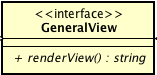
\includegraphics[scale=0.5]{Sezioni/SottosezioniST/img/app/GeneralView.png}
	\caption{feature::GeneralView}
\end{figure}

\begin{itemize}
\item \textbf{Descrizione}: Interfaccia che sta alla base della gerarchia delle componenti della lista-spesa.
\item \textbf{Utilizzo}:
\item \textbf{Attributi}: 
\item \textbf{Metodi}:
	\begin{itemize}
	\item \textit{public renderView():string}\\
	Genera il codice HTML CSS JS necessario per visualizzare una componente grafica della lista-spesa.
	\end{itemize}
\item \textbf{Eventi}:
\end{itemize}

\subsubsection{feature::remove\_item::RemoveItemView}

\label{feature::remove_item::RemoveItemView}
\begin{figure}[H]
	\centering
	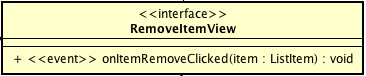
\includegraphics[scale=0.5]{Sezioni/SottosezioniST/img/app/RemoveItemView.png}
	\caption{feature::remove\_item::RemoveItemView}
\end{figure}

\begin{itemize}
\item \textbf{Descrizione}: Questa interfaccia rappresenta la view relativa alla rimozione di un oggetto dalla lista-spesa.
\item \textbf{Utilizzo}: L'interfaccia viene utilizzata per disaccoppiare presenter e implementazione della rimozione, visualizza i dati che gli vengono passati dal presenter.
\item \textbf{Attributi}: 
\item \textbf{Metodi}:
\item \textbf{Eventi}:
	\begin{itemize}	
	\item \textit{public onItemRemoveClicked(item:ListItem):void}\\
	Evento che rappresenta il click, da parte dell'utente, sull'oggetto visuale necessario alla rimozione di un oggetto dalla lista.
			\\ \textbf{Parametri}: \begin{itemize}
			\item \textit{item:ListItem}\\
			L'oggetto che è stato cliccato e che l'utente desidera rimuoverlo dalla lista.
			\end{itemize} 
	\end{itemize}
\end{itemize}

\subsubsection{feature::remove\_item::view::RemoveItemViewImpl}

\label{feature::remove_item::view::RemoveItemViewImpl}
\begin{figure}[H]
	\centering
	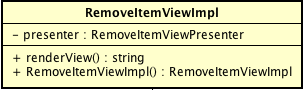
\includegraphics[scale=0.5]{Sezioni/SottosezioniST/img/app/RemoveItemViewImpl.png}
	\caption{feature::remove\_item::view::RemoveItemViewImpl}
\end{figure}

\begin{itemize}
\item \textbf{Descrizione}: Questa classe rappresenta la vista per la rimozione di un oggetto dalla lista-spesa, implementando l'interfaccia RemoveItemView.
\item \textbf{Utilizzo}: Questa classe viene utilizzata dall'utente ogniqualvolta vuole rimuovere un oggetto alla lista-spesa.
\item \textbf{Attributi}: 
	\begin{itemize}
	\item \textit{private presenter:RemoveItemViewPresenter}\\
	Il presenter associato alla rimozione di un oggetto della lista, al quale questa classe delega la gestione del comportamento dell'elemento di rimozione degli oggetti.
	\end{itemize}
\item \textbf{Metodi}:
	\begin{itemize}
	\item \textit{public renderView():string}\\
		Genera il codice HTML CSS JS necessario per visualizzare la componente grafica della lista-spesa necessaria alla rimozione di un oggetto da essa.
	\item \textit{public RemoveItemViewImpl():RemoveItemViewImpl}\\
	Costruttore della classe RemoveItemViewImpl.
	\end{itemize}
\item \textbf{Eventi}:
\end{itemize}

\subsubsection{feature::remove\_item::presenter::RemoveItemViewPresenter}

\label{feature::remove_item::presenter::RemoveItemViewPresenter}
\begin{figure}[H]
	\centering
	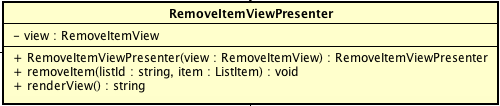
\includegraphics[scale=0.5]{Sezioni/SottosezioniST/img/app/RemoveItemViewPresenter.png}
	\caption{feature::remove\_item::presenter::RemoveItemViewPresenter}
\end{figure}

\begin{itemize}
\item \textbf{Descrizione}: Questa classe rappresenta il presenter per gli elementi di rimozione degli oggetti  della lista-spesa.
\item \textbf{Utilizzo}: Il presenter fa da tramite tra l'implementazione dell'elemento di rimozione e la view, formattando i dati che verranno visualizzati nella view e manipolando gli input dell'utente per eseguire le operazioni predisposte.
\item \textbf{Attributi}: 
	\begin{itemize}
	\item \textit{private view:RemoveItemView}\\
	La view associata al presenter.
	\end{itemize}
\item \textbf{Metodi}:
	\begin{itemize}
	\item \textit{RemoveItemViewPresenter(view:RemoveItemView):RemoveItemViewPresenter}\\
	Costruttore della classe RemoveItemViewPresenter.
			\\ \textbf{Parametri}: \begin{itemize}
			\item \textit{view:RemoveItemView}\\
			La view necessaria alla costruzione del presenter.
			\end{itemize} 
	\item \textit{public removeItem(listId:string,item:ListItem):void}\\
	Questo metodo serve per rimuovere un oggetto dalla lista-spesa.
			\\ \textbf{Parametri}: \begin{itemize}
			\item \textit{listId:string}\\
			L'id della lista dalla quale bisogna rimuovere l'oggetto.
			\item \textit{item:ListItem}\\
			L'oggetto da rimuovere.
			\end{itemize} 
	\item \textit{public renderView():string}\\
	Genera il codice HTML CSS JS necessario per visualizzare la componente grafica della lista-spesa necessaria alla rimozione di un oggetto da essa.
	\end{itemize}
\item \textbf{Eventi}:
\end{itemize}

\subsubsection{usecase::ModifyListUseCase}

\label{usecase::ModifyListUseCase}
\begin{figure}[H]
	\centering
	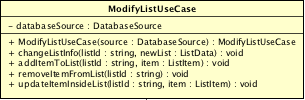
\includegraphics[scale=0.5]{Sezioni/SottosezioniST/img/app/ModifyListUseCase.png}
	\caption{usecase::ModifyListUseCase}
\end{figure}

\begin{itemize}
\item \textbf{Descrizione}: La classe rappresenta l'interazione con il database nel caso di modifiche alla lista.
\item \textbf{Utilizzo}: Ogni modifica dei dati degli oggetti della lista o della lista stessa passa per questa classe, che fa ponte tra il presenter e il database.
\item \textbf{Attributi}: 
	\begin{itemize}
	\item \textit{private databaseSource:DatabaseSource}\\
	Questo attributo è un riferimento all'interfaccia \texttt{DatabaseSource}, che permette di interfacciarsi al database \termine{MongoDB}.
	\end{itemize}
\item \textbf{Metodi}:
	\begin{itemize}
	\item \textit{public ModifyListUseCase(source:DatabaseSource):ModifyListUseCase}\\
	Costruttore della classe ModifyListUseCase.
			\\ \textbf{Parametri}: \begin{itemize}
			\item \textit{source:DatabaseSource}\\
			Attributo necessario alla costruzione della classe, per la comunicazione con  il database.
			\end{itemize} 
	\item \textit{public changeListInfo(listId:string,newList:ListData):void}\\
	Questo metodo serve per modificare i dati di una lista.
			\\ \textbf{Parametri}: \begin{itemize}
			\item \textit{listId:string}\\
			L'id della lista che si vuole modificare.
			\item \textit{newList:ListData}\\
			La nuova lista che si andrà a sostituire alla precedente.
			\end{itemize} 
	\item \textit{public addItemToList(listId:string,item:ListItem):void}\\
	Metodo che aggiunge un oggetto a una lista-spesa.
			\\ \textbf{Parametri}: \begin{itemize}
			\item \textit{listId:string}\\
			Id della lista alla quale si vuole aggiungere un oggetto.
			\item \textit{item:ListItem}\\
			Oggetto che si vuole aggiungere alla lista.
			\end{itemize} 
	\item \textit{public removeItemFromList(listId:string, itemId : string):void}\\
	Metodo che rimuove un oggetto da una list-spesa.
			\\ \textbf{Parametri}: \begin{itemize}
			\item \textit{listId:string}\\
			Id della lista dalla quale si vuole rimuovere un oggetto.
			\item \textit{itemId : string} \\
			Id dell'oggetto che si vuole rimuovere dalla lista
			\end{itemize} 
	\item \textit{public updateItemInsideList(listId:string,item:ListItem):void}\\
	Metodo che modifica un oggetto della lista.
			\\ \textbf{Parametri}: \begin{itemize}
			\item \textit{listId:string}\\
			Id della lista della quale si vuole modificare un oggetto.
			\item \textit{item:ListItem}\\
			Oggetto che si vuole sostituire all'oggetto della lista con id dato.
			\end{itemize} 
	\end{itemize}
\item \textbf{Eventi}:
\end{itemize}

\subsubsection{database::DatabaseSource}

\label{database::DatabaseSource}
\begin{figure}[H]
	\centering
	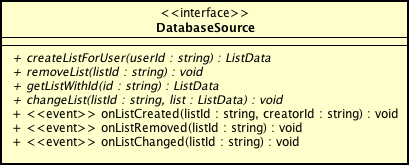
\includegraphics[scale=0.5]{Sezioni/SottosezioniST/img/app/DatabaseSource.png}
	\caption{database::DatabaseSource}
\end{figure}

\begin{itemize}
\item \textbf{Descrizione}: Interfaccia che permette la comunicazione tra il model ed il database sul quale verranno salvati tutti i dati relativi alle varie liste. I metodi da essa esposti non vengono descritti nel dettaglio in quanto l'implementazione di questa interfaccia utilizzerà i noti metodi di Meteor.js, descritti approfonditamente nella rispettiva documentazione inserita all'interno dei riferimenti normativi.
\item \textbf{Utilizzo}: Interfaccia che permette di salvare, modificare, rimuovere dati all'interno del database.
\item \textbf{Attributi}: 
\item \textbf{Metodi}:
	\begin{itemize}
	\item \textit{public createListForUser(userId:string):ListData}\\
		Crea all'interno del database una nuova lista per l'utente impostato e ritorna tale lista.
			\\ \textbf{Parametri}: \begin{itemize}
			\item \textit{userId:string}\\
			Utente per cui verrà creata una nuova lista.
			\end{itemize} 
	\item \textit{public removeList(listId:string):void}\\
	Rimuove all'interno del database la lista con l'id indicato.
			\\ \textbf{Parametri}: \begin{itemize}
			\item \textit{listId:string}\\
				Id della lista da rimuovere dal database.
			\end{itemize} 
	\item \textit{public getListWithId(id:string):ListData}\\
	Restituisce la lista con l'id indicato recuperandola dal database.
			\\ \textbf{Parametri}: \begin{itemize}
			\item \textit{id:string}\\
			Id della lista di cui recuperare i dati dal database.
			\end{itemize} 
	\item \textit{public changeList(listId:string, list:ListData):void}\\
		Permette di modificare i dati e le informazioni di una lista all'interno del database.
			\item{\textbf{Parametri}: \begin{itemize}
			\item \textit{listId:string}\\
			Id della lista di cui si vogliono modificare i dati o le informazioni.
			\item \textit{list:ListData}\\
			Insieme dei dati e informazioni che verranno sostituiti a quelli esistenti per la relativa lista.
			\end{itemize}}
	\end{itemize}
\item \textbf{Eventi}:
	\begin{itemize}
	\item \textit{public onListCreated(listId:string,creatorId:string):void}\\
		Evento che notifica tutti gli oggetti in ascolto che la lista è stata creata nel database.
			\\ \textbf{Parametri}: \begin{itemize}
			\item \textit{listId:string}\\
			Id della lista appena creata nel database.
			\item \textit{creatorId:string}\\
			Id dell'utente creatore della lista.
			\end{itemize} 
	\item \textit{public onListRemoved(listId:string,creatorId:string):void}\\
			Evento che notifica tutti gli oggetti in ascolto che la lista è stata rimossa dal database.
			\\ \textbf{Parametri}: \begin{itemize}
			\item \textit{listId:string}\\
			Id della lista appena rimossa.
			\end{itemize} 
	\item \textit{public onListChanged(listId:string):void}\\
				Evento che notifica tutti gli oggetti in ascolto che la lista è stata modificata nel database.
			\\ \textbf{Parametri}: \begin{itemize}
			\item \textit{listId:string}\\
			Id della lista modificata all'interno del database.
			\end{itemize} 
	\end{itemize}
\end{itemize}

\subsubsection{feature::add\_item::AddItemView}

\label{feature::add_item::AddItemView}
\begin{figure}[H]
	\centering
	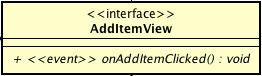
\includegraphics[scale=0.5]{Sezioni/SottosezioniST/img/app/AddItemView.png}
	\caption{feature::add\_item::AddItemView}
\end{figure}

\begin{itemize}
\item \textbf{Descrizione}: Questa interfaccia rappresenta la view relativa all'aggiunta di un oggetto alla lista-spesa.
\item \textbf{Utilizzo}: L'interfaccia viene utilizzata per disaccoppiare presenter e implementazione dell'aggiunta, visualizza i dati che gli vengono passati dal presenter.
\item \textbf{Attributi}: 
\item \textbf{Metodi}:
\item \textbf{Eventi}:
	\begin{itemize}	
	\item \textit{public onAddItemClicked():void}\\
	Evento che rappresenta il click, da parte dell'utente, sull'oggetto visuale necessario all'aggiunta di un oggetto alla lista.
	\end{itemize}
\end{itemize}

\subsubsection{feature::add\_item::view::AddItemViewImpl}

\label{feature::add_item::view::AddItemViewImpl}
\begin{figure}[H]
	\centering
	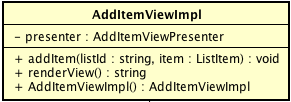
\includegraphics[scale=0.5]{Sezioni/SottosezioniST/img/app/AddItemViewImplementation.png}
	\caption{feature::add\_item::view::AddItemViewImpl}
\end{figure}

\begin{itemize}
\item \textbf{Descrizione}: Questa classe rappresenta l'aggiunta di un oggetto alla lista-spesa, implementando l'interfaccia AddItemView.
\item \textbf{Utilizzo}: Questa classe viene utilizzata dall'utente ogniqualvolta vuole aggiungere un oggetto alla lista-spesa.
\item \textbf{Attributi}: 
	\begin{itemize}
	\item \textit{private presenter:AddItemViewPresenter}\\
	Il presenter associato all'aggiunta di un oggetto della lista, al quale questa classe delega la gestione del comportamento dell'elemento di aggiunta degli oggetti.
	\end{itemize}
\item \textbf{Metodi}:
	\begin{itemize}
	\item \textit{public addItem(listId:string,item:ListItem):void}\\
	Il metodo aggiunge un oggetto a una lista-spesa.
			\\ \textbf{Parametri}: \begin{itemize}
			\item \textit{listId:string}\\
			L'id della lista al quale si vuole aggiungere un oggetto.
			\item \textit{item:ListItem}\\
			L'oggetto che si vuole aggiungere alla lista.
			\end{itemize} 
	\item \textit{public renderView():string}\\
	Genera il codice HTML CSS JS necessario per visualizzare la componente grafica della lista-spesa necessaria all'aggiunta di un oggetto da essa.
	\item \textit{AddItemViewImpl():AddItemViewImpl}\\
	Il costruttore della classe AddItemViewImpl.
	\end{itemize}
\item \textbf{Eventi}:
\end{itemize}

\subsubsection{feature::add\_item::presenter::AddItemViewPresenter}

\label{feature::add_item::presenter::AddItemViewPresenter}
\begin{figure}[H]
	\centering
	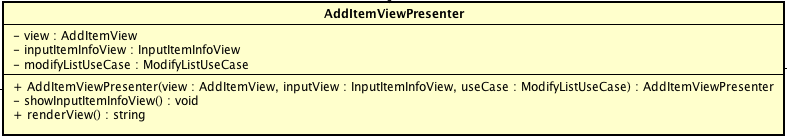
\includegraphics[scale=0.5]{Sezioni/SottosezioniST/img/app/AddItemViewPresenter.png}
	\caption{feature::add\_item::presenter::AddItemViewPresenter}
\end{figure}

\begin{itemize}
\item \textbf{Descrizione}: Questa classe rappresenta il presenter per gli elementi di rimozione degli oggetti  della lista-spesa.
\item \textbf{Utilizzo}: Il presenter fa da tramite tra l'implementazione dell'elemento di aggiunta e la view, formattando i dati che verranno visualizzati nella view e manipolando gli input dell'utente per eseguire le operazioni predisposte.
\item \textbf{Attributi}: 
	\begin{itemize}
	\item \textit{private view:AddItemView}\\
	La view associata al presenter.
	\item \textit{private inputItemInfoView:InputItemInfoView}\\
	Componente grafica per l'input dei dati relativi a un oggetto della lista-spesa.
	\item \textit{private modifyListUseCase:ModifyListUseCase}\\
	Componente necessaria alla comunicazione tra presenter e database.
	\end{itemize}
\item \textbf{Metodi}:
	\begin{itemize}
	\item \textit{public AddItemViewPresenter(view:AddItemView, inputView:InputItemInfoView, \\ useCase:ModifyListUseCase):AddItemViewPresenter}\\
	Il costruttore della classe AddItemViewPresenter.	
		\item{\textbf{Parametri}: \begin{itemize}
		\item \textit{view:AddItemView}\\
			La view associata al presenter.
		\item \textit{inputView:InputItemInfoView}\\
			Componente grafica per l'input dei dati relativi a un oggetto della lista-spesa.
		\item \textit{useCase:ModifyListUseCase}\\
			Componente necessaria alla comunicazione tra presenter e database.
		\end{itemize}}
	\item \textit{private showInputItemInfoView():void}\\
	Mostra la componente grafica necessaria all'input dei dati per un oggetto della lista-spesa.
	\item \textit{public renderView():string}\\
	Genera il codice HTML CSS JS necessario per visualizzare la componente grafica della lista-spesa necessaria all'aggiunta di un oggetto da essa.
	\end{itemize}
\item \textbf{Eventi}:
\end{itemize}

\subsubsection{usecase::ShowPopupUseCase}

\label{usecase::ShowPopupUseCase}
\begin{figure}[H]
	\centering
	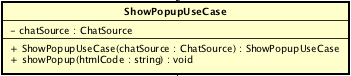
\includegraphics[scale=0.5]{Sezioni/SottosezioniST/img/app/ShowPopupUseCase.png}
	\caption{usecase::ShowPopupUseCase}
\end{figure}

\begin{itemize}
\item \textbf{Descrizione}: La classe rappresenta una utility per la creazione facilitata di popup.
\item \textbf{Utilizzo}: La classe viene utilizzata ogniqualvolta una delle altre classi necessita di mostrare un modale nelle sue interazioni.
\item \textbf{Attributi}: 
	\begin{itemize}
	\item \textit{private chatSource:ChatSource}\\
	Interfaccia che permette la comunicazione con la chat all'interno della quale si vuole mostrare il popup.
	\end{itemize}
\item \textbf{Metodi}:
	\begin{itemize}
	\item \textit{public showPopup(htmlCode:string):void}\\
	Questo metodo mostra un modale.
			\\ \textbf{Parametri}: \begin{itemize}
			\item \textit{htmlCode:string}\\
			La stringa contiene il codice HTML del contenuto del modale che si vuole mostrare.
			\end{itemize} 
	\item \textit{ShowPopupUseCase(chatSource:ChatSource):ShowPopupUseCase}\\
	Costruttore della classe ShowPopupUseCase.
		\\\textbf{Parametri}: \begin{itemize}
		\item \textit{chatSource:ChatSource}\\
		Chat necessaria alla costruzione della classe.
		\end{itemize} 
	\end{itemize}
\item \textbf{Eventi}:
\end{itemize}

\subsubsection{communication::ChatSource}

\label{communication::ChatSource}
\begin{figure}[H]
	\centering
	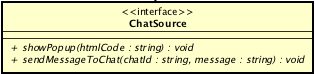
\includegraphics[scale=0.5]{Sezioni/SottosezioniST/img/app/ChatSource.png}
	\caption{communication::ChatSource}
\end{figure}

\begin{itemize}
\item \textbf{Descrizione}: Interfaccia che permette la comunicazione con l'istanza di Rocket.chat.  I metodi messi a disposizione da questa interfaccia non vengono descritti nel dettaglio in quanto verranno implementati attraverso l'utilizzo di metodi descritti già approfonditamente dettagliati all'interno della documentazione di Rocket.chat stesso che è possibile trovare visitando la rispettiva pagina web il quale collegamento è stato inserito all'interno dei riferimenti informativi.
\item \textbf{Utilizzo}: Permette di mostrare popup e inviare messaggi o effettuare altre operazioni riguardanti la chat.
\item \textbf{Attributi}: 
\item \textbf{Metodi}:
	\begin{itemize}
	\item \textit{public showPopup(htmlCode:string):void}\\
	Permette di visualizzare un popup che contiene il codice html dato.
			\\\textbf{Parametri}: \begin{itemize}
			\item \textit{htmlCode:string}\\
				Codice HTML che verrà visualizzato nel popup.
			\end{itemize} 
			\item \textit{public sendMessageToChat(chatId:string, message:string):void}\\
			Permette di inviare un messaggio alla chat impostata.
			\\ \textbf{Parametri}: \begin{itemize}
			\item \textit{chatId:string}\\
			Id della chat a cui inviare verrà inviato il messaggio.
			\item \textit{message:string}\\
			Messaggio che verrà inviato alla chat.
\end{itemize} 
	\end{itemize}
\item \textbf{Eventi}:
\end{itemize}